%%%%%%%%%%%%%%%%%%%%%%%%%%%%%%%%%%%%%%%%%%%%%%%%%%%%%%%%%%%%%%%
%% BRIEF VERSION OF OXFORD THESIS TEMPLATE FOR CHAPTER PREVIEWS

%%%%% CHOOSE PAGE LAYOUT
% format for PDF output (ie equal margins, no extra blank pages):
\documentclass[a4paper,nobind]{templates/ociamthesis}

% UL 30 Nov 2018 pandoc puts lists in 'tightlist' command when no space between bullet points in Rmd file
\providecommand{\tightlist}{%
  \setlength{\itemsep}{0pt}\setlength{\parskip}{0pt}}
  
 \usepackage[utf8]{inputenc}
% UL 1 Dec 2018, fix to include code in shaded environments
\usepackage{color}
\usepackage{fancyvrb}
\newcommand{\VerbBar}{|}
\newcommand{\VERB}{\Verb[commandchars=\\\{\}]}
\DefineVerbatimEnvironment{Highlighting}{Verbatim}{commandchars=\\\{\}}
% Add ',fontsize=\small' for more characters per line
\usepackage{framed}
\definecolor{shadecolor}{RGB}{248,248,248}
\newenvironment{Shaded}{\begin{snugshade}}{\end{snugshade}}
\newcommand{\AlertTok}[1]{\textcolor[rgb]{0.94,0.16,0.16}{#1}}
\newcommand{\AnnotationTok}[1]{\textcolor[rgb]{0.56,0.35,0.01}{\textbf{\textit{#1}}}}
\newcommand{\AttributeTok}[1]{\textcolor[rgb]{0.77,0.63,0.00}{#1}}
\newcommand{\BaseNTok}[1]{\textcolor[rgb]{0.00,0.00,0.81}{#1}}
\newcommand{\BuiltInTok}[1]{#1}
\newcommand{\CharTok}[1]{\textcolor[rgb]{0.31,0.60,0.02}{#1}}
\newcommand{\CommentTok}[1]{\textcolor[rgb]{0.56,0.35,0.01}{\textit{#1}}}
\newcommand{\CommentVarTok}[1]{\textcolor[rgb]{0.56,0.35,0.01}{\textbf{\textit{#1}}}}
\newcommand{\ConstantTok}[1]{\textcolor[rgb]{0.00,0.00,0.00}{#1}}
\newcommand{\ControlFlowTok}[1]{\textcolor[rgb]{0.13,0.29,0.53}{\textbf{#1}}}
\newcommand{\DataTypeTok}[1]{\textcolor[rgb]{0.13,0.29,0.53}{#1}}
\newcommand{\DecValTok}[1]{\textcolor[rgb]{0.00,0.00,0.81}{#1}}
\newcommand{\DocumentationTok}[1]{\textcolor[rgb]{0.56,0.35,0.01}{\textbf{\textit{#1}}}}
\newcommand{\ErrorTok}[1]{\textcolor[rgb]{0.64,0.00,0.00}{\textbf{#1}}}
\newcommand{\ExtensionTok}[1]{#1}
\newcommand{\FloatTok}[1]{\textcolor[rgb]{0.00,0.00,0.81}{#1}}
\newcommand{\FunctionTok}[1]{\textcolor[rgb]{0.00,0.00,0.00}{#1}}
\newcommand{\ImportTok}[1]{#1}
\newcommand{\InformationTok}[1]{\textcolor[rgb]{0.56,0.35,0.01}{\textbf{\textit{#1}}}}
\newcommand{\KeywordTok}[1]{\textcolor[rgb]{0.13,0.29,0.53}{\textbf{#1}}}
\newcommand{\NormalTok}[1]{#1}
\newcommand{\OperatorTok}[1]{\textcolor[rgb]{0.81,0.36,0.00}{\textbf{#1}}}
\newcommand{\OtherTok}[1]{\textcolor[rgb]{0.56,0.35,0.01}{#1}}
\newcommand{\PreprocessorTok}[1]{\textcolor[rgb]{0.56,0.35,0.01}{\textit{#1}}}
\newcommand{\RegionMarkerTok}[1]{#1}
\newcommand{\SpecialCharTok}[1]{\textcolor[rgb]{0.00,0.00,0.00}{#1}}
\newcommand{\SpecialStringTok}[1]{\textcolor[rgb]{0.31,0.60,0.02}{#1}}
\newcommand{\StringTok}[1]{\textcolor[rgb]{0.31,0.60,0.02}{#1}}
\newcommand{\VariableTok}[1]{\textcolor[rgb]{0.00,0.00,0.00}{#1}}
\newcommand{\VerbatimStringTok}[1]{\textcolor[rgb]{0.31,0.60,0.02}{#1}}
\newcommand{\WarningTok}[1]{\textcolor[rgb]{0.56,0.35,0.01}{\textbf{\textit{#1}}}}

%UL 2 Dec 2018 add a bit of white space before and after code blocks
\renewenvironment{Shaded}
{
  \vspace{4pt}%
  \begin{snugshade}%
}{%
  \end{snugshade}%
  \vspace{4pt}%
}
%UL 2 Dec 2018 reduce whitespace around verbatim environments
\usepackage{etoolbox}
\makeatletter
\preto{\@verbatim}{\topsep=0pt \partopsep=0pt }
\makeatother

%UL 28 Mar 2019, enable strikethrough
\usepackage[normalem]{ulem}

%UL 3 Nov 2019, avoid mysterious error from not having hyperref included
\usepackage{hyperref}

%%%%% SELECT YOUR DRAFT OPTIONS
% Three options going on here; use in any combination.  But remember to turn the first two off before
% generating a PDF to send to the printer!

% This adds a "DRAFT" footer to every normal page.  (The first page of each chapter is not a "normal" page.)

% This highlights (in blue) corrections marked with (for words) \mccorrect{blah} or (for whole
% paragraphs) \begin{mccorrection} . . . \end{mccorrection}.  This can be useful for sending a PDF of
% your corrected thesis to your examiners for review.  Turn it off, and the blue disappears.

%%%%% BIBLIOGRAPHY SETUP
% Note that your bibliography will require some tweaking depending on your department, preferred format, etc.
% The options included below are just very basic "sciencey" and "humanitiesey" options to get started.
% If you've not used LaTeX before, I recommend reading a little about biblatex/biber and getting started with it.
% If you're already a LaTeX pro and are used to natbib or something, modify as necessary.
% Either way, you'll have to choose and configure an appropriate bibliography format...

% The science-type option: numerical in-text citation with references in order of appearance.
% \usepackage[style=numeric-comp, sorting=none, backend=biber, doi=false, isbn=false]{biblatex}
% \newcommand*{\bibtitle}{References}

% The humanities-type option: author-year in-text citation with an alphabetical works cited.
% \usepackage[style=authoryear, sorting=nyt, backend=biber, maxcitenames=2, useprefix, doi=false, isbn=false]{biblatex}
% \newcommand*{\bibtitle}{Works Cited}

%UL 3 Dec 2018: set this from YAML in index.Rmd
\usepackage[style=numeric-comp, sorting=none, backend=biber, doi=false, isbn=false]{biblatex}
\newcommand*{\bibtitle}{References}

% This makes the bibliography left-aligned (not 'justified') and slightly smaller font.
\renewcommand*{\bibfont}{\raggedright\small}

% Change this to the name of your .bib file (usually exported from a citation manager like Zotero or EndNote).
\addbibresource{references.bib}

%%%%% YOUR OWN PERSONAL MACROS
% This is a good place to dump your own LaTeX macros as they come up.

% To make text superscripts shortcuts
	\renewcommand{\th}{\textsuperscript{th}} % ex: I won 4\th place
	\newcommand{\nd}{\textsuperscript{nd}}
	\renewcommand{\st}{\textsuperscript{st}}
	\newcommand{\rd}{\textsuperscript{rd}}

%%%%% THE ACTUAL DOCUMENT STARTS HERE
\begin{document}

%%%%% CHOOSE YOUR LINE SPACING HERE
% This is the official option.  Use it for your submission copy and library copy:
\setlength{\textbaselineskip}{22pt plus2pt}
% This is closer spacing (about 1.5-spaced) that you might prefer for your personal copies:
%\setlength{\textbaselineskip}{18pt plus2pt minus1pt}

% UL: You can set the general paragraph spacing here - I've set it to 2pt (was 0) so
% it's less claustrophobic
\setlength{\parskip}{2pt plus 1pt}

% Leave this line alone; it gets things started for the real document.
\setlength{\baselineskip}{\textbaselineskip}

% all your chapters and appendices will appear here
\hypertarget{APD-study}{%
\chapter{APD study}\label{APD-study}}

\chaptermark{APD study}

\minitoc 

\hypertarget{introduction}{%
\section{Introduction}\label{introduction}}

\hypertarget{methods}{%
\section{Methods}\label{methods}}

\hypertarget{participants}{%
\subsection{Participants}\label{participants}}

Forty-four primary school children native British English speakers with
normal hearing acuity participated in the study. Amongst them 20
belonged to the APD clinical group (5 females) with an average age of
11.04 \(\pm\)~1.42 years (range: 7.8 - 12.9 years). One APD child was
excluded from the analysis due to raised thresholds
(PTA\textgreater25~dB~HL). APD children were recruited in two ways.
Children diagnosed with APD at Great Ormond Street Hospital (GOSH) and
at the London Hearing and Balance Centre (LHBC), London, UK, and
fulfilled the recruitment criteria were identified and contacted by a
clinical team member. The parents/caregivers were provided with
information about the study and means of contact to express interest in
participation. Others were recruited by advertisements in social
networks, where parents were requested to fill-out an interest form that
included screening questions to ensure they fulfil the participation
requirements. {To add percentage for clinics, diagnosed/LiD/susAPD and
SPD pattern?} The remaining 23 (12 females) comprised of typically
developing control children (TD) with no reported concerns or diagnosis
of a language or other cognitive developmental disorders. The TD group
average age was 9.47 \(\pm\)~1.58 years and ranged between 7 to 12.1
years (A detailed description of the groups is shown in Tab. ??).

Difference in variance for age between the two groups was tested using
t-test with Welch degrees of freedom correction for uneven sample-size,
showing a significant difference in age between the groups
{[}t(40.95)=3.43, p=0.001{]}.

The project was approved by the UCL Research Ethics Committee (Project
ID Number 0544/006) and the NHS Health Research Authority HRA (REC
reference: 18/LO/0250). The testing commenced once an informed consent
was given by both the parent/caregiver and the child.

\begin{itemize}
\tightlist
\item
  Background questionnaire
\item
  Otoscopic examination was carried out to ensure the eardrum is
  visible, healthy and intact.
\item
  Location of the testing
\item
  duration of the session
\end{itemize}

Participants from both TD and APD group completed the same battery of
tests listed below

\hypertarget{auditory-evaluation}{%
\subsection{Auditory evaluation}\label{auditory-evaluation}}

\hypertarget{standard-audiometry}{%
\subsubsection{\texorpdfstring{\textbf{Standard
audiometry}}{Standard audiometry}}\label{standard-audiometry}}

\begin{figure}

{\centering \includegraphics[width=0.85\linewidth]{03-rmd-basics-cites-and-refs_files/figure-latex/PTA-1} 

}

\caption{APD participants pure-tone audiogram thresholds for standard frequencies plotted for the left and the right ear (black). The shaded grey area represents the TD group range of audiometric thresholds and the white line represents the mean at each frequency. The dashed line represents the threshold criteria of hearing level $\leq$ 25 dB HL.}\label{fig:PTA}
\end{figure}

A standard air conduction pure-tone audiometric evaluation at
\(\frac{1}{3}\) octave band frequencies ranging between 0.25 to 8~kHz
was carried out using ???? audiometer and ??? headphones. Normal hearing
acuity was defined by thresholds \(\leq\) 25~dB~HL for frequencies
ranging from 0.25 to 4~kHz. Thresholds at 8~kHz were \(\leq\) 25~dB~HL
for all the participants, excluding two participants with measured
thresholds at 35 and 30~dB~HL in one ear, respectively. The listeners'
thresholds for the left and the right ear are plotted in Figure
@ref(fig:PTA). The shaded grey area represents the TD group thresholds
range and the white line represents their mean at each frequency. The
black lines represents the individual thresholds in the APD group and
the group mean is marked by the bold black line. The dashed line
represents the maximal thresholds criteria \(\leq\) 25~dB~HL for normal
hearing.

{Results belong here??}

\hypertarget{extended-high-frequency-audiometry-ehfa}{%
\subsubsection{Extended high-frequency audiometry
(EHFA)}\label{extended-high-frequency-audiometry-ehfa}}

Extended high-frequency pure-tone audiometry was carried out at four
\(\frac{1}{3}\) octave band frequencies 8, 11, 16, \& 20~kHz using a
locally developed MATLAB based software which generated and collected
the data. Measurements took place at SHaPS, UCL laboratory in an
electromagnetically shielded sound proof booth which is typically used
for EEG measurements. A Windows PC situated outside the booth was
connected via USB to an RME ???? sound card (Audio AG, Haimhausen
Germany) and an ER10X Extended-Bandwidth Acoustic Probe System
(Etym\(\bar{o}\)tic Research, Elk Grove Village, IL) which was located
in the testing booth. Once the ear probe was placed in the child's ear,
an in-situ sound pressure level calibration was performed (chirp noise)
using a MATLAB code provided by ????.

Speak with KZ about the measurements

\hypertarget{switching-task-st}{%
\subsubsection{Switching task (ST)}\label{switching-task-st}}

The switching task (ST) is a novel speech-on-speech listening task that
involves perception of interrupted and periodically segmented speech
that is switched between the two ears out-of-phase with an interrupted
distractor. Since segments of the target and of the distractor are never
presented in the same ear at the same time, it enables to eliminate
peripheral (EM) masking, while maintaining high IM for speech
distractors. The task assesses the ability to switch attention and
integration of binaural information.

Refer to Chapter 2 and briefly describe the stimuli and difference in
the methods.

As described in Chapter 2 Section ???, two test versions were used with
varying in sentence structure and complexity: 1. ASL 2. CCRM

Masker Types..

\hypertarget{spatialised-speech-in-noise-lisns-uk}{%
\subsubsection{Spatialised speech-in-noise
(LiSNS-UK)}\label{spatialised-speech-in-noise-lisns-uk}}

The Listening in Spatialised Noise Sentences UK (LiSNS-UK) assesses the
ability to use binaural cues in speech-on-speech listening conditions.
The test development, speech material normalisation, and norms
standardisation followed Cameron and Dillon (2007) development steps and
are described in detail in Chapter ???. The test uses virtualisation
techniques to create spatial distribution of sound sources in space for
headphones presentation where target sentences (ASL; MacLeod and
Summerfield 1990) are presented in two simultaneous speech distractors
(unrelated children's stories spoken by the target talker). It comprises
of two main listening conditions, differing in their availability of
spatial cues. The target sentences are configured to always appear in
front of the listener's head, at 0\(^{\circ}\) azimuth on the horizontal
plane, with the two streams of speech distractors either co-located in
space with the target (S0N0), resulting in relatively poor speech
perception, or offset in space, with one distractor to either side of
the target at \(\pm\)~90\(^{\circ}\), resulting in an improvement in
speech perception of circa 13~dB (Cameron, Glyde, and Dillon 2011),
typically termed as spatial release from masking (SRM). This SRM
advantage is calculated by taking the difference between performance in
the co-located condition and the separated condition. The speech
distractors were presented continuously throughout a run at a fixed
65?~dB~SPL output level and comprised of a combination of two out of
three different passages children stories. A 1-up/1-down adaptive
procedure was used, varying the level of the target talker relative to
the distractors depending on listener's correct/incorrect response to
measure the listeners' speech reception threshold (SRT), i.e., the
signal-to-noise-ratio (SNR) yielding 50\% speech intelligibility. A 2~ms
long 1~kHz pure-tone was presented 500~ms before the target sentence
onset at 65?~dB~SPL (0 dB SNR) as a reference cue signalling the
listener to attend the coming target sentence. The initial target output
level was ??~dB~SPL with an initial step-size of 4~dB SNR. The step-size
was reduced after every reversal, reaching a minimum step-size of
2~dB~SNR after three practice reversals. A stopping rule was introduced
in case the maximal SNR was reached more than three times and the
procedure was considered to be successfully completed in case test
reversals were obtained. The SRT was then calculated by averaging test
reversals SNRs (i.e., following three practice reversals). Each run
consisted of 25 sentences taken from 8? phonemically-balanced test list
which were constructed following the normalisation of the speech. In
addition, a sentence-specific level correction was applied to the target
signal (see Chapter ?? for more information). The order of the listening
condition, test lists, target sentences and distractors combinations was
fixed across all the participants and started with the collocated
condition. Spatialisation was applied by convolving each stimuli with
head-related transfer functions (HRTFs) at the corresponding azimuthal
direction separately for the left and the right channel. The HRTFs were
measured with a Knowles Electronics Manikin for Acoustic Research
(KEMAR, REF) manikin with a small pinnae taken from the CIPIC HRTF
database\footnote{The database is available online in:
  \url{https://www.ece.ucdavis.edu/cipic/spatial-sound/hrtf-data/}}
{[}Algazi et al. (2001); see ``special'' HRTF data{]}. A
post-equalisation step was applied in order to flatten the magnitude of
the headphones frequency response. Headphone-to-ear Transfer Functions
(HpTFs) measured with KEMAR manikin for HD-25 supraaural headphones were
extracted from Wierstorf et al. (2011) HRTF database. The final mixed
stimulus was filtered with the inverse HpTFs separately for the left and
the right channel before being combined together as a final step. Every
participant was presented with two runs, one for each listening
condition (collocated/separated). Testing started following a practice
phase of two runs for each of the test conditions with five BKB
sentences each (Bench, Kowal, and Bamford 1979). Listeners were
instructed to verbally repeat the target sentences to the experimenter
who was situated alongside the participant in a sound treated chamber.
The experimenter scored the response by selecting the correctly repeated
keywords on the screen. Listeners were encouraged to guess if unsure
while no feedback was given at any time. A loose keyword scoring method
was used, whereby errors of case or declension were considered as
correct responses. For example, a repetition of the keywords
`\(<\)clown\emph{s}\(>\) \(<\)funny\(>\) \(<\)face\emph{s}\(>\)' to the
stimulus `The \(<\)clown\(>\) had a \(<\)funny\(>\) \(<\)face\(>\)'.

\hypertarget{speech-in-noise-spin}{%
\subsubsection{Speech-in-noise (SPIN)}\label{speech-in-noise-spin}}

The speech-in-noise test was used as a more realistic listening
situation that is widely used in the clinic as opposed to more complex
listening tasks as listed above. The normalised ASL sentences were
presented in a speech-shaped-noise (SSN) with spectrum matched to the
ASL corpus. The SSN onset was 500~ms before the target sentence begin.
The exact same adaptive proccedure as for the LiSNS-UK was used with the
same stop-rules. Each listenr was presented with a single run of 25
sentences following a practice phase with seven BKB sentences. The same
test list and sentences order was used across all the listeners.

\hypertarget{the-environmental-auditory-scene-analysis-task-envasa}{%
\subsubsection{The Environmental Auditory Scene Analysis task
(ENVASA)}\label{the-environmental-auditory-scene-analysis-task-envasa}}

In analogy to the classic `cocktail-party' scenario, ENVASA is a
non-linguistic paradigm (Leech et al. 2009) that measures detection of
everyday environmental sounds presented in naturalistic auditory scenes
and can be used to asses IM effects as well as sustained selective
auditory attention skills. In the task, short environmental target
sounds (e.g., a ``dog's bark'', ``door knock'' or ``bouncing ball'')
were presented in a dichotic background scene (i.e., the target sound is
presented only in one ear) consisting of either a single background
scene,presented in both ears, or two background scenes, each presented
in a different ear. The number of targets, the onset time and
presentation ear varied across trials. Four target/background SNRs were
employed split into two categories `low' (-6 and -3~dB) and `high' (0
and +3~dB) by varying the target level. Target/background contextual
agreement was manipulated by embedding the target sound in a
\emph{congruent} background scene that is in agreement with the
listener's expectations (e.g., a cow's `moo' in a farmyard scene) or in
an \emph{incongruent} background scene which violate these expectations
(e.g., a cow's `moo' in a traffic scene).

Procedure:

The experiment was carried out using the original code and laptop as
used and described by Leech et al. (2009). Sounds were presented via
Sennheiser HD-25 headphones (REF) and the participants response was
recorded using ???? gamepad. The output level was adjusted to a
comfortable level before the test started. The participants were
situated in front of the laptop placed on a desk and were instructed to
hold the gamepad. Prior to the test begin the listeners were presented
with a short child-friendly video covering the task's instructions and
demonstrated two test trials. Following the instruction video, the
examiner gave the child a short recap of the task's instructions and
simulated with the child an exemplary trial to make sure the child is
familiarised with the task. The task began with three practice trials
with provided feedback, while no further feedback was given in the
testing phase.

Every trial was made of two parts, starting with a target audio and
visual familiarisation phase before the main target detection phase.
Target identification was recorded by pressing one of the three buttons
on the gamepad which corresponded to the location of the target objects
on the screen. A response was counted as correct only if the
participants pushed the corresponding button within 2~s time interval,
300~ms following the target onset. The outcome measure was calculated as
the percentage of target sounds correctly identified within a condition
(\%-correct).

In total there were 92 target sounds presented over 40 trials, with half
of the target sounds presented in a single- and half in a
dual-background condition. In Occasional foil target items were played
at 0~dB~SNR without a corresponding picture on the screen and were used
to estimate the quality of the participants performance. Each target
item was served once as a foil item and their order was randomised.

(ref:Leech2009) Schematic of the ENVASA experimental paradigm (taken
from Leech et al. 2009)

\begin{figure}

{\centering 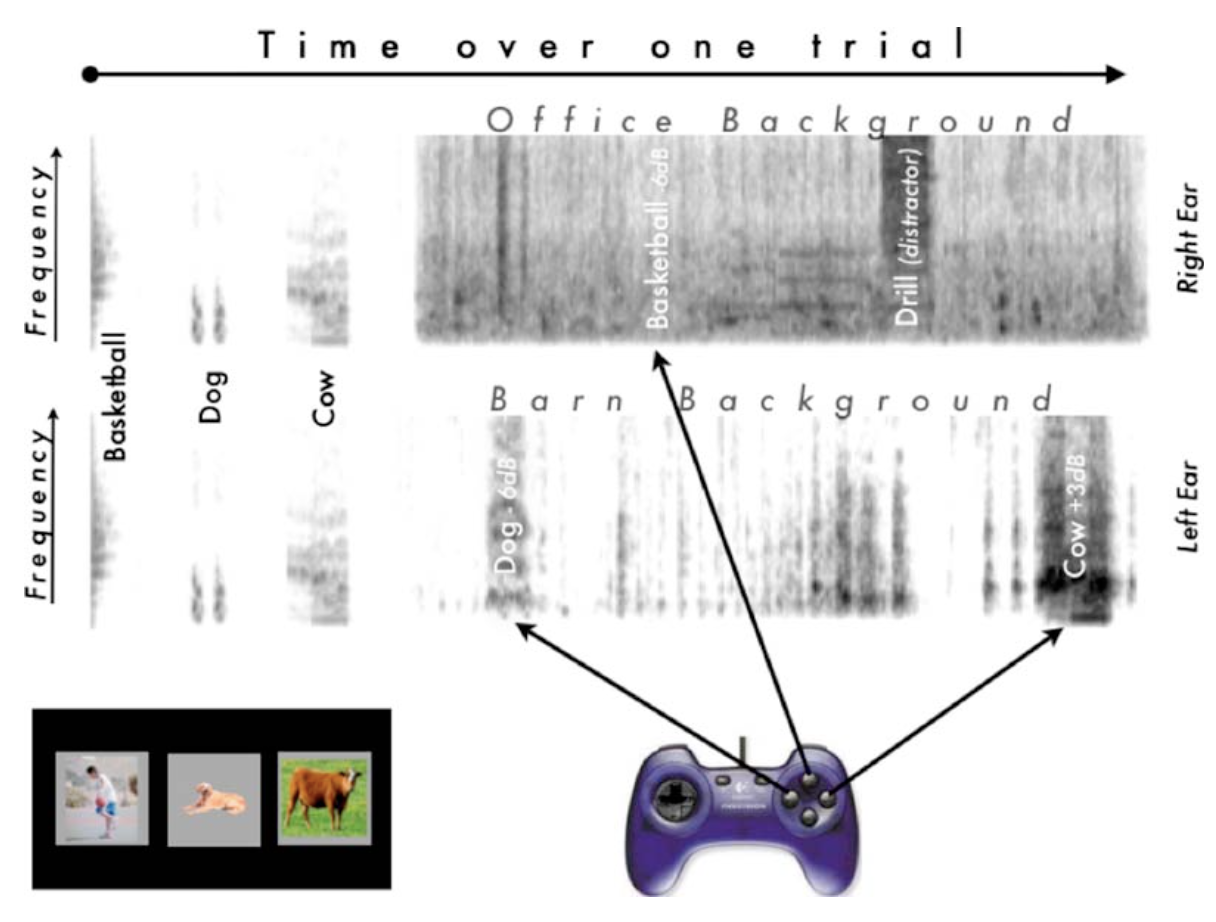
\includegraphics[width=0.65\linewidth]{figures/ENVASAparadigm} 

}

\caption{(ref:Leech2009)}\label{fig:ENVASA}
\end{figure}

\hypertarget{celf-rs}{%
\subsubsection{CELF-RS}\label{celf-rs}}

The Recalling Sentences (RS) sub-test of the Clinical Evaluation of
Language Fundamentals Fifth UK edition (CELF-5-UK H Wiig, Semel, and
Secord 2017) was administered to assess the listeners expressive
language ability and has been shown to be a good indicator of the
listeners general language skills (REF). In the task the child is
presented with pre-recorded sentences of increasing length and
complexity and required to repeat sentences without any changes. Scoring
were marked by hand by the examiner as instructed by the test manual.
The sentences were spoken by a standard southern British English female
and were recorded in a sound-treated recording booth at the SHaPS UCL
laboratory, London. The sentences were presented using a MATLAB program
via headphones using the same experimental equipment as listed above at
a comfortable output level of 70~dB~HL. The task began with two practice
sentences while the number of test items varied depending on the child's
age performance. No repetitions or feedback was given during the testing
and the test was discontinued in case the child failed to score any
points for four consecutive items. Age-scaled score were calculated
based on the test norms whereby the cut-off scaled score for abnormal
performance is \(\leq\)~7. Average scaled score are between 8 to 12
(\(\pm\)~1~SD) while scores \(\geq\)~13 (+1~SD)are classified as above
average.

\hypertarget{questionnaires}{%
\subsection{Questionnaires}\label{questionnaires}}

\hypertarget{medical-neurological-and-pysiological-history}{%
\subsubsection*{Medical, Neurological, and Pysiological
History}\label{medical-neurological-and-pysiological-history}}
\addcontentsline{toc}{subsubsection}{Medical, Neurological, and
Pysiological History}

\hypertarget{the-evaluation-pf-childrens-listening-and-processing-skills-eclips}{%
\subsubsection*{The Evaluation pf Children's Listening and Processing
Skills
(ECLiPS)}\label{the-evaluation-pf-childrens-listening-and-processing-skills-eclips}}
\addcontentsline{toc}{subsubsection}{The Evaluation pf Children's
Listening and Processing Skills (ECLiPS)}

The ECLiPS questionnaire (Barry and Moore 2014) comprises of 38 items
where the users are asked to express their agreement simple statements
about the child's listening and other related skills or behaviours using
a five-point Likert scale (from ``strongly agree'' to ``strongly
disagree''). The ECLiPS was design to identify listening and
communication difficulties in children aged 6 to 11 years. Nonetheless,
the UK standardisation study (REF) found little to no age effect on
scores in many of the scale items, suggesting the testing age could be
extended below and beyond the population used for the development. Based
on factor analysis the items are grouped into five subcategories: 1.
Speech \& Auditory Processing (SAP), 2. Environmental \& Auditory
Sensitivity (EAS), 3. Language, literacy \& laterality (L/L/L), 4.
Memory \& Attention (M\&A), 5. Pragmatic \& Social skills (PSS). Age-
and sex-scaled scores were computed using the test excel scorer.

A score below the 10\(^{th}\) percentile (corresponding to a scale score
of circa 6) is generally considered clinically significant.

\hypertarget{the-childrens-communication-checklist-2nd-edition-ccc-2}{%
\subsubsection*{\texorpdfstring{The Children's Communication Checklist
2\(^{nd}\) edition
(CCC-2)}{The Children's Communication Checklist 2\^{}\{nd\} edition (CCC-2)}}\label{the-childrens-communication-checklist-2nd-edition-ccc-2}}
\addcontentsline{toc}{subsubsection}{The Children's Communication
Checklist 2\(^{nd}\) edition (CCC-2)}

Communication abilities were assessed using the Children's Communication
Checklist second edition questionnaire (CCC-2; D. V. M. 2003) was
completed by the child's parent/guardian. The CCC-2 was designed to
screen communication problems in children aged 4 to 16 years and
comprises of 70 checklist items each comprising of a behaviour statement
like ``Mixes up words of similar meaning''. The respondents are asked to
judge how often the behaviours occur using a four-point Likert rating
scale: 0. \emph{less than once a week (or never)}, 1. \emph{at least
once a week, but not every day}, 2. \emph{once or twice a day}, 3.
\emph{several times (more than twice) a day (or always)}. The items are
grouped into ten sub-scales of behaviours tapping into different skills
(A. Speech, B. Syntax, C. Semantics, D. Coherence, E. Inappropriate
initiation, F. Stereotyped language, G. Use of context, H. Non-verbal
communication, I. Social relations, J. Interests). Taking the sum of
scores for the sub-scales A to H are used to derive the General
Communication Composite (GCC) which is used to identify clinically
abnormal communication competence. A GCC score \textless{} 55 was found
by Norbury and BIshop (2005) to well separate between control and
clinical groups, identifying children with scores at the bottom 10\%.
Another composite (Social-Interaction Deviance Composite, SIDC) was
taken by taking the difference in sum of scales E, H, I, and J from the
sum of scales of A to D. Abnormal GCC (\textless~55) combined with a
negative SIDC score has been shown to be indicative of an autistic
spectrum disorder profile (D. V. M. 2003). The CCC-2 scaled and
composite scores were computed using the test excel scorer. X
observations out of Y were removed from the analysis due to inconsistent
reports flagged by the test scorer.

\hypertarget{results}{%
\section{Results}\label{results}}

\hypertarget{extended-high-frequency-audiometry-ehfa-1}{%
\subsection{Extended high-frequency audiometry
(EHFA)}\label{extended-high-frequency-audiometry-ehfa-1}}

The listeners' thresholds for the left and the right ear are plotted in
Figure @ref(fig:EHF). The shaded grey area represents the TD group
thresholds range and the white line represents their mean at each
frequency. The black lines represents the individual thresholds in the
APD group and the group mean is marked by the bold black line.

{Difference in HL between audiogram types?} First, the quality(?) of the
thresholds measured with the non-standard ER10X audiogram was tested by
comparing the individuals thresholds with those obtained with the
standard audiometer. This was tested group-wise for thresholds at 8~kHz
measured in the left and the right ear using Wilcoxon signed rank test
for paired samples (rstatix::wilcox\_test with bonferroni adjustment;
REF). The test showed a significant difference in thresholds between the
two audiogram type for the TD group in both right (p=1, effect size
r=0.114) and the left ear (p=1, r=0.092). No significant difference was
found in the APD group in both ears (right: p=0.544, r=0.235; left:
p=0.844, r=0.2).

{Difference between groups} Similarly, difference in thresholds between
the groups across frequencies (11 \& 16~kHz) and ears (left/right) was
tested using a Wilcoxon rank-sum test for unpaired samples
(rstatix::wilcox\_test with bonferroni adjustment; REF). No significant
difference was found between the groups for all frequency/ear
combinations (all p\textgreater.05).

{PTAs and BEs}

The same holds for PTAs (calculated as the mean of thresholds at 11 \&
16~kHz, severalty for the left and the right ear) as well as for PTA at
the better ear, where no significant difference was found between the
groups. This was tested using a Wilcoxon rank-sum test for unpaired
samples with permutation (coin::wilcox\_test, REF).

\begin{figure}

{\centering \includegraphics[width=0.85\linewidth]{03-rmd-basics-cites-and-refs_files/figure-latex/EHF-1} 

}

\caption{APD participants pure-tone thresholds for extended high-frequencies plotted for the left and the right ear (black). The shaded grey area represents the TD group range of audiometric thresholds and the white line represents the mean at each frequency..}\label{fig:EHF}
\end{figure}

\hypertarget{switching-task-st-1}{%
\subsection{Switching task (ST)}\label{switching-task-st-1}}

\begin{itemize}
\tightlist
\item
  Describe how data was inspected and corrected for outliers
\end{itemize}

\hypertarget{asl}{%
\subsubsection{ASL}\label{asl}}

\hypertarget{ccrm}{%
\subsubsection{CCRM}\label{ccrm}}

\hypertarget{spatialised-speech-in-noise-lisns-uk-1}{%
\subsection{Spatialised speech-in-noise
(LiSNS-UK)}\label{spatialised-speech-in-noise-lisns-uk-1}}

\begin{table}

\caption{\label{tab:LiSNS-uRevs}Add caption here...}
\centering
\begin{tabular}[t]{lrrrrrrrrrr}
\toprule
\multicolumn{1}{c}{ } & \multicolumn{5}{c}{TD} & \multicolumn{5}{c}{APD} \\
\cmidrule(l{3pt}r{3pt}){2-6} \cmidrule(l{3pt}r{3pt}){7-11}
condition & n & mean & sd & min & max & n & mean & sd & min & max\\
\midrule
SSN & 23 & -5.31 & 1.42 & -8.05 & -2.00 & 20 & -4.82 & 1.36 & -7.4 & -2.30\\
S0N0 & 23 & -1.79 & 1.90 & -5.55 & 2.95 & 20 & -1.81 & 1.74 & -4.7 & 2.37\\
S0N90 & 23 & -9.07 & 2.55 & -13.50 & -3.42 & 20 & -9.02 & 2.70 & -13.8 & -1.70\\
SRM & 23 & 7.28 & 1.21 & 4.20 & 9.17 & 20 & 7.22 & 2.46 & 1.0 & 11.40\\
\bottomrule
\end{tabular}
\end{table}

Descriptive statistics of the listeners performance split across the two
groups is given in Tab. ??. A total of two SRTs were obtained for each
participant, one for the spatially collocated (S0N0) and one for the
spatially separated (S0N90) listening condition. In addition, the
listeners' SRM was calculated by taking the difference between the two
conditions (SRM = S0N0 - S0N90).

see Table @ref(tab:LiSNS-uRevs)

\hypertarget{speech-in-noise-spin-1}{%
\subsection{Speech-in-noise (SPIN)}\label{speech-in-noise-spin-1}}

\hypertarget{the-environmental-auditory-scene-analysis-task-envasa-1}{%
\subsection{The Environmental Auditory Scene Analysis task
(ENVASA)}\label{the-environmental-auditory-scene-analysis-task-envasa-1}}

\begin{figure}

{\centering \includegraphics[width=1\linewidth]{03-rmd-basics-cites-and-refs_files/figure-latex/ENVASA-plots1-1} 

}

\caption{Add caption here}\label{fig:ENVASA-plots1}
\end{figure}

Initial inspection of the individuals performance was performed to
ensure that the task instructions were followed and well understood.
Performance for the reference condition (single incongruent background
at a high SNR), which is expected to least impact performance, was
compared with a cut-off criterion of 56~\%, calculated as 2 standard
deviations from the TD group mean (84~\% \(\pm\)~14~\%). Individuals
with performance bellow the cut-off criterion were excluded from the
analysis. One TD group aged 7 years old who scored 45~\% was thus
excluded. Of the remaining data 20 belonged to the TD group and 17 to
the APD group.

Due to the small number of observations in each condition and for
clarity, \%-correct was calculated for three measures: i. a \emph{single
background}, ii. a \emph{dual backgrounds}, iii. and a \emph{combined}
measure where scores in both conditions were summed together\footnote{See
  Appendix ?? for a more detailed summary of the listeners scores split
  into the different test condition.}. Visual inspection of the
listeners scores as a function of age (see Figure
@ref(fig:ENVASA-plots1)) showed a developmental trend in performance.
This was suppurated by Kendall rank correlation test for non-parametric
data with small sample-size, where performance significantly improved
with increased age across the groups in all three measures
(p~\textless~.05), excluding the APD group for single background
(p~=~0.096; see the complete test results in Figure
@ref(fig:ENVASA-plots1)). This is in agreement with Krishnan et al.
(2013) study where they found a strong developmental effect across
normal-hearing typically developing children in a similar age range to
those measured in the present study.

Thus, further analysis, age was controlled for using the same
multiple-case approach method described in ????. The individuals scores
were transformed into z-scores based on standard residuals estimated
from a linear regression model fitted from the TD data only. To account
for outliers TD children with scores the TD data used by the model was

\begin{verbatim}
## Warning in grid.Call.graphics(C_text, as.graphicsAnnot(x$label), x$x, x$y, :
## conversion failure on 'better performance →' in 'mbcsToSbcs': dot substituted
## for <e2>
\end{verbatim}

\begin{verbatim}
## Warning in grid.Call.graphics(C_text, as.graphicsAnnot(x$label), x$x, x$y, :
## conversion failure on 'better performance →' in 'mbcsToSbcs': dot substituted
## for <86>
\end{verbatim}

\begin{verbatim}
## Warning in grid.Call.graphics(C_text, as.graphicsAnnot(x$label), x$x, x$y, :
## conversion failure on 'better performance →' in 'mbcsToSbcs': dot substituted
## for <92>
\end{verbatim}

\begin{figure}

{\centering \includegraphics[width=1\linewidth]{03-rmd-basics-cites-and-refs_files/figure-latex/ENVASA-plots2-1} 

}

\caption{Add caption here}\label{fig:ENVASA-plots2}
\end{figure}

\begin{itemize}
\item
  Test for age effect
\item
  z-transformed scores
\item
  Group difference: Wilcoxon rank-sum test with permutation
\item
  Correlation with other measures
\end{itemize}

For appendix:

\begin{itemize}
\tightlist
\item
  similar figure to Kirshnan's figure with \% correct \& scores by age
  \& z-scores
\end{itemize}

\hypertarget{celf-rs-1}{%
\subsection{CELF-RS}\label{celf-rs-1}}

\hypertarget{questionnaires-1}{%
\subsection{Questionnaires}\label{questionnaires-1}}

\hypertarget{discussion}{%
\section{Discussion}\label{discussion}}

\hypertarget{conclusion}{%
\section{Conclusion}\label{conclusion}}

\clearpage

\hypertarget{refs}{}
\begin{cslreferences}
\leavevmode\hypertarget{ref-Algazi2001}{}%
Algazi, V. R., R. O. Duda, D. M. Thompson, and Carlosa Avendano. 2001.
``The CIPIC HRTF database.'' In \emph{IEEE Assp Workshop on Applications
of Signal Processing to Audio and Acoustics}.
\url{https://doi.org/10.1109/aspaa.2001.969552}.

\leavevmode\hypertarget{ref-Barry2014}{}%
Barry, Johanna G., and David R. Moore. 2014. ``Evaluation of Children's
Listening and Processing Skills (ECLiPS).'' London, United Kingdom:
MRC-T.

\leavevmode\hypertarget{ref-Bench1979}{}%
Bench, John, Åse Kowal, and John Bamford. 1979. ``The Bkb
(Bamford-Kowal-Bench) Sentence Lists for Partially-Hearing Children.''
\emph{British Journal of Audiology} 13 (3): 108--12.
\url{https://doi.org/10.3109/03005367909078884}.

\leavevmode\hypertarget{ref-Cameron2007}{}%
Cameron, Sharon, and Harvey Dillon. 2007. ``Development of the Listening
in Spatialized Noise-Sentences Test (LISN-S).'' \emph{Ear and Hearing}
28 (2): 196--211. \url{https://doi.org/10.1097/AUD.0b013e318031267f}.

\leavevmode\hypertarget{ref-Cameron2011}{}%
Cameron, Sharon, Helen Glyde, and Harvey Dillon. 2011. ``Listening in
Spatialized Noise---Sentences Test (LiSN-S): Normative and Retest
Reliability Data for Adolescents and Adults up to 60 Years of Age.''
\emph{Journal of the American Academy of Audiology} 22 (10): 697--709.
\url{https://doi.org/10.3766/jaaa.22.10.7}.

\leavevmode\hypertarget{ref-D.V.M.2003}{}%
D. V. M., Bishop. 2003. ``The Children's Communication Checklist,
Version 2 (CCC-2).'' London, United Kingdom: The Psycho- logical
Corporation.

\leavevmode\hypertarget{ref-HWiig2017}{}%
H Wiig, Elisabeth, Eleanor Semel, and Wayne Secord. 2017. ``Clinical
Evaluation of Language Fundamentals - Fifth Edition UK (CELF-5UK).''
PsychCorp, Pearson Clinical Assessment.

\leavevmode\hypertarget{ref-Krishnan2013}{}%
Krishnan, Saloni, Robert Leech, Jennifer Aydelott, and Frederic Dick.
2013. ``School-age children's environmental object identification in
natural auditory scenes: Effects of masking and contextual congruence.''
\emph{Hearing Research} 300: 46--55.
\url{https://doi.org/10.1016/j.heares.2013.03.003}.

\leavevmode\hypertarget{ref-Leech2009}{}%
Leech, Robert, Brian Gygi, Jennifer Aydelott, and Frederic Dick. 2009.
``Informational factors in identifying environmental sounds in natural
auditory scenes.'' \emph{The Journal of the Acoustical Society of
America} 126 (6): 3147--55. \url{https://doi.org/10.1121/1.3238160}.

\leavevmode\hypertarget{ref-MacLeod1990}{}%
MacLeod, A, and Q Summerfield. 1990. ``A procedure for measuring
auditory and audiovisual speech-reception thresholds for sentences in
noise: Rationale, evaluation, and recommendations for use.''
\emph{British Journal of Audiology} 24 (October): 29--43.
\url{https://doi.org/10.3109/03005369009077840}.

\leavevmode\hypertarget{ref-Norbury2005}{}%
Norbury, Courtenay Frazier, and Dorothy V M BIshop. 2005. ``Children ' s
Communication Checklist - 2 : a validation study.'' \emph{Publie Dans
Revue Tranel} 42: 53--63.

\leavevmode\hypertarget{ref-Wierstorf2011}{}%
Wierstorf, Hagen, Matthias Geier, Alexander Raake, and Sascha Spors.
2011. ``A Free Database of Head-Related Impulse Response Measurements in
the Horizontal Plane with Multiple Distances.'' In \emph{AES130}.
\end{cslreferences}


%%%%% REFERENCES

% JEM: Quote for the top of references (just like a chapter quote if you're using them).  Comment to skip.
% \begin{savequote}[8cm]
% The first kind of intellectual and artistic personality belongs to the hedgehogs, the second to the foxes \dots
%   \qauthor{--- Sir Isaiah Berlin \cite{berlin_hedgehog_2013}}
% \end{savequote}

\setlength{\baselineskip}{0pt} % JEM: Single-space References

{\renewcommand*\MakeUppercase[1]{#1}%
\printbibliography[heading=bibintoc,title={\bibtitle}]}

\end{document}
